\chapter{Implementierung}
	\section{Temperatur-/Feuchtigkeitssensor HYT2x1}
		\subsection{Anschluss}
			Beide Sensoren, sowohl HYT241 als auch HYT271, verfügen über vier Anschlusspins. Die zwei äußeren Pins sind VCC und GND. Die inneren Pins sind SDA und SCL, welche für die Übertragung per I$^{2}$C zuständig sind.
			
			SDA dient zur Datenübertragung. SCL ist der Taktanschluss, der standardmäßig mit einer Frequenz von 100 kHz betrieben wird. Optional hätten auch 400 kHz zur Verfügung gestanden, wurden jedoch nicht benutzt da im vorliegen Projekt keine höheren Datenraten nötig waren.
			
			Das mbed Entwicklungsboard verfügt über zwei I$^{2}$C Bus Anschlüsse. Genutzt wird der Bus auf Pin9 und Pin10. Der Schaltplan diesbezüglich kann in Abbildung \ref{fig:HYT_Schalt} betrachtet werden.
			
			\begin{figure}[H]
				\centering
				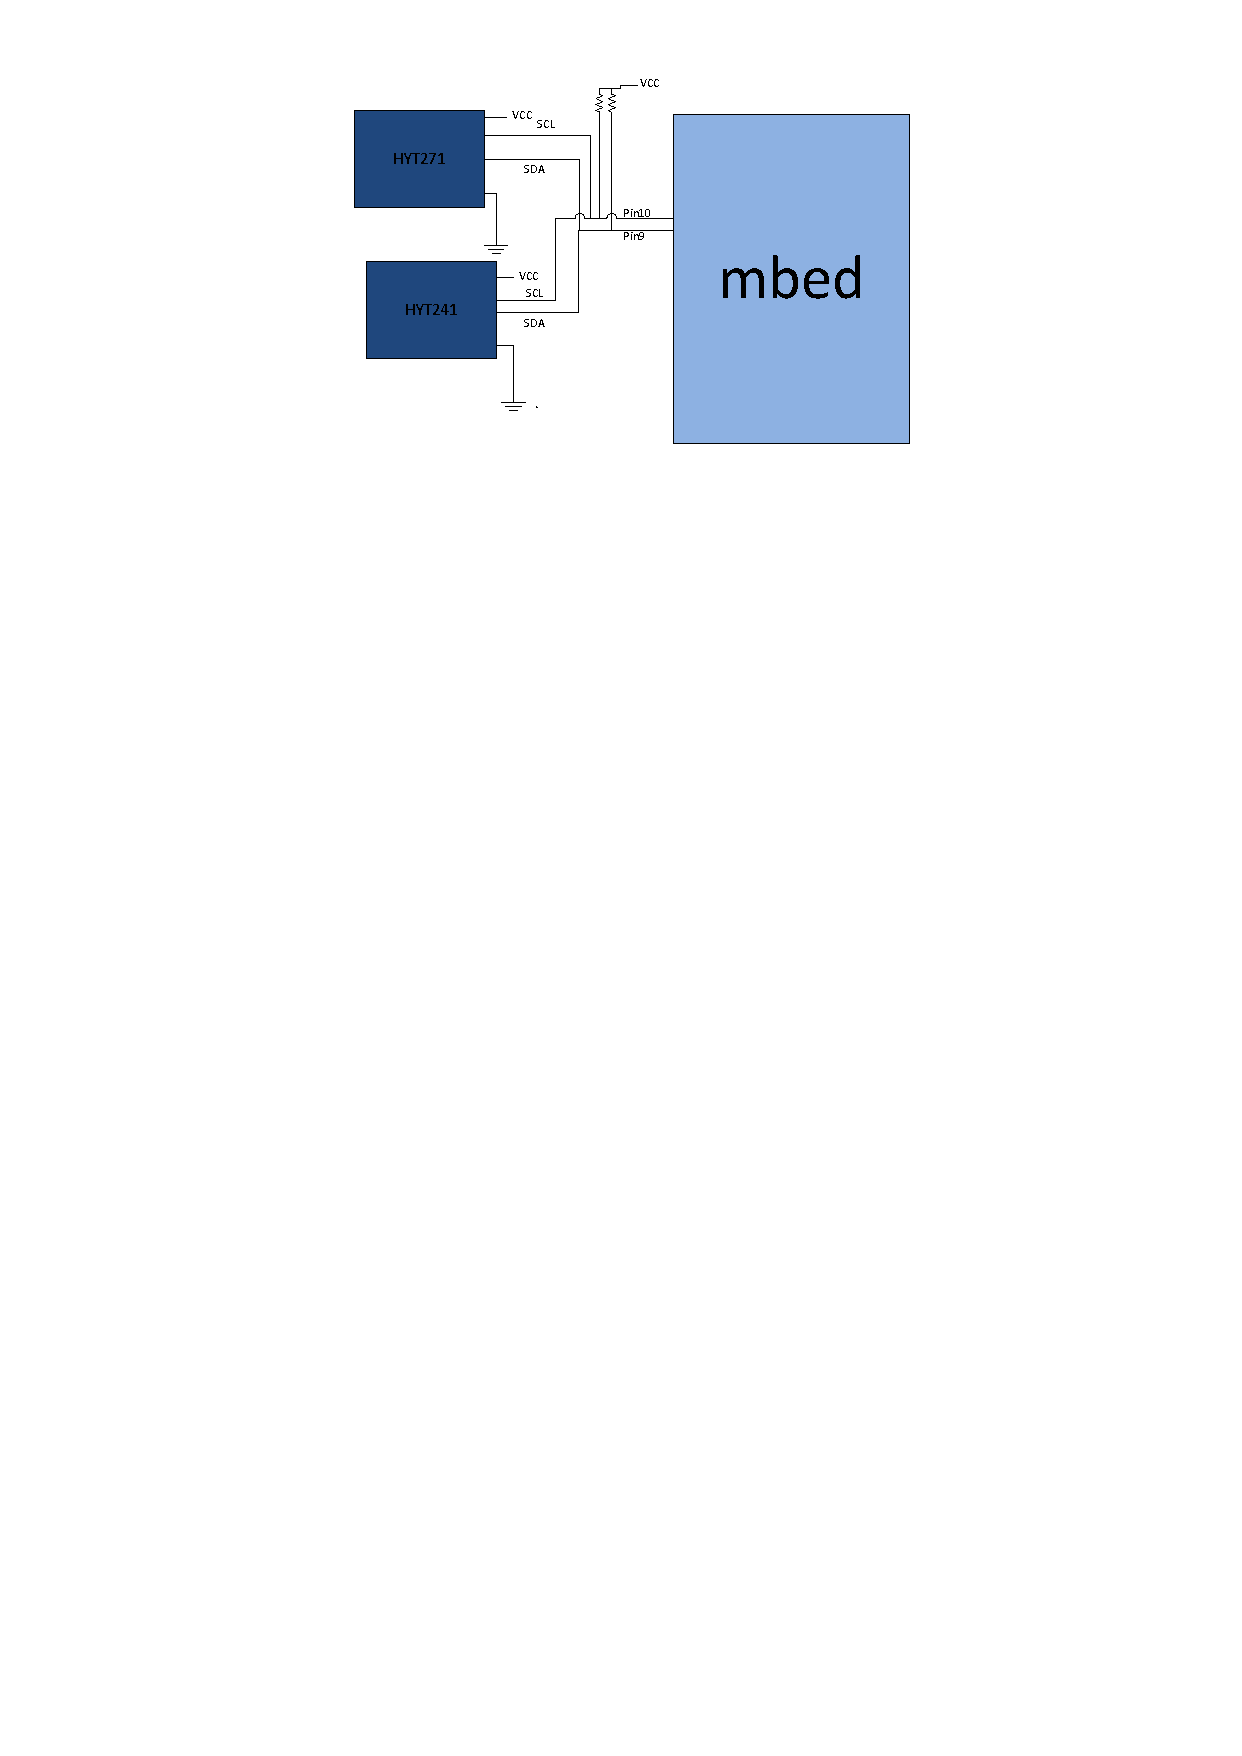
\includegraphics[width=\textwidth]{Schaltplaene/HYT_I2C}
				\caption{Schaltplan bezüglich der Temperatur-/Feuchtigkeitssensoren}
				\label{fig:HYT_Schalt}
			\end{figure}

		\subsection{Adressen}
			Im Projekt werden zwei Sensoren über einen Bus angesteuert. Das heißt, dass beide Sensoren mit Pin9 und Pin10 verbunden sind. Sie besitzen allerdings die gleiche Standardadresse 0x28. Damit beide Sensoren korrekt arbeiten musste die Adresse des HYT241 auf 0x20 geändert werden. Die extra Schaltung, die hierfür nötig war ist in Abbildung \ref{fig:HYT_Schalt_Umprog} zu sehen.
			
			\begin{figure}[H]
				\centering
				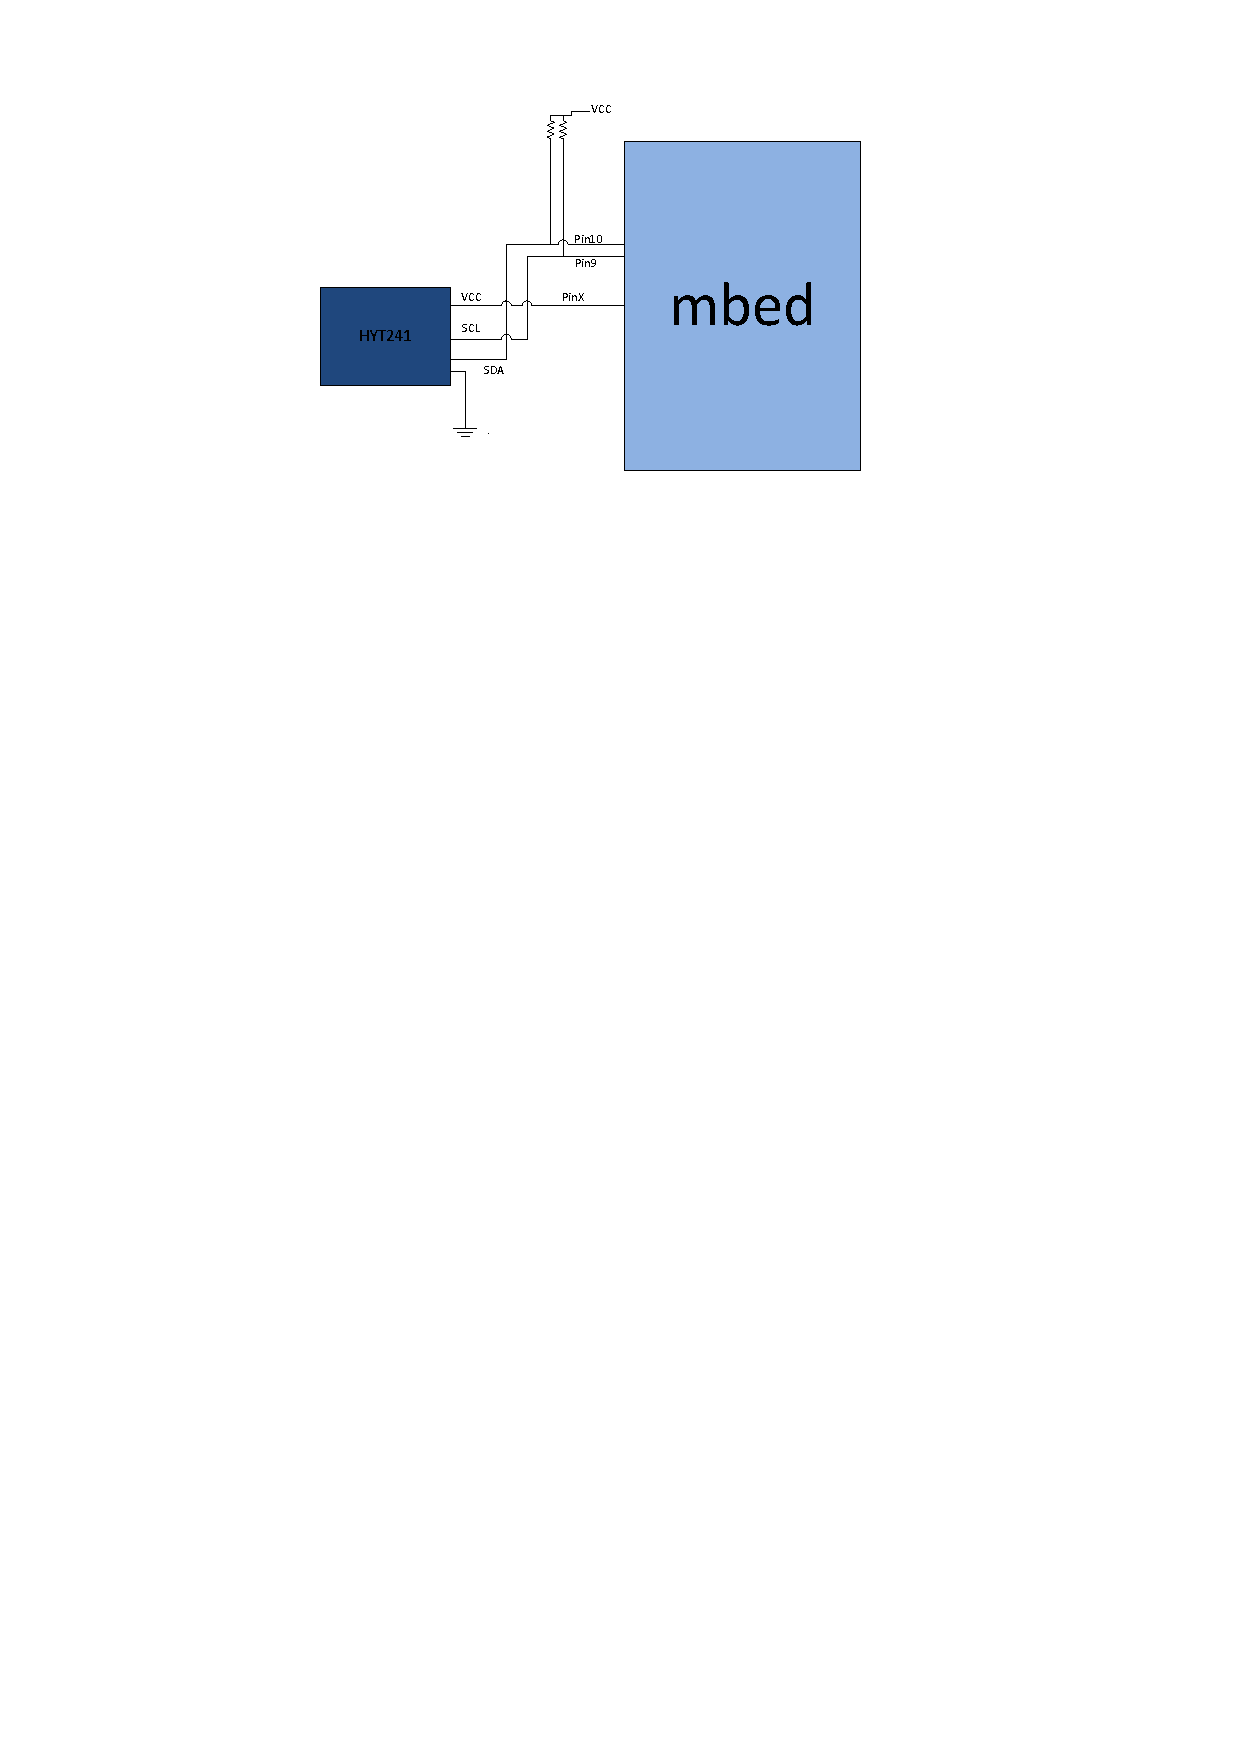
\includegraphics[width=\textwidth]{Schaltplaene/Umprogrammieren}
				\caption{Schaltplan bezüglich der Adressänderung}
				\label{fig:HYT_Schalt_Umprog}
			\end{figure}

			\subsubsection{Das Adressänderungsprotokoll}
			Innerhalb der ersten 10 ms nach dem einschalten des Sensors kann dieser in den Programmiermodus gesetzt werden. Da dieses Zeitfenster mit dem mbed Entwicklungsboard jedoch schlecht zu treffen ist musste zum verändern der Adresse die Schaltung selbst verändert werden, damit der Sensor separat eingeschaltet werden kann.
			
			Zunächst muss der VCC Pin des Sensors mit einem beliebigen freien Pin des mbed Prototypboards verbunden werden. Dann kann die Methode setAdress() der HYT2x1 Klasse aufgerufen werden.
			
			\newpage
			Durch das Aufrufen der setAdress() Methode wird der VCC Pin des Sensors auf High\footnote{Eigentlich reichen Logikausgänge nicht aus um Sensoren mit Strom zu versorgen, da ihre Leistung schlicht zu gering ist. Im Falle des HYT241 spielt das jedoch keine Rolle. Dieser ist so sparsam ausgelegt das auch ein Logikausgang ausreicht um ihn mit Strom zu versorgen.} gelegt. Durch das Anlegen des High-Signals wird der Sensor eingeschaltet und man kann ihn in den Programmiermodus setzen. Dazu muss der Befehl \{0xA0,0x00,0x00\} auf die bisherige Adresse des Sensors geschrieben werden. Da man dem Sensor etwas Zeit geben muss den Befehl zu bearbeiten, wird anschließend 100ms gewartet. Dann kann der nächste Befehl gesendet werden. Dieser lautet \{0x5C,0x00,Adresse\footnote{Die neue Adresse im Hexadezimalen Format.}\}. Folgend muss erneut 100ms gewartet werden. Jetzt muss nur noch der letzte Befehl zum Bestätigen der Adresse gesendet werden, der \{0x80,0x00,0x00\} lautet. Nun wurde die Adresse des Sensors geändert, wodurch er nicht mehr auf die alte Adresse reagiert.
			
			Anmerkung: Dieses Protokoll steht nicht im Datenblatt des Sensors und wurde über mehrere Forenbeiträge aus dem Internet zusammengetragen. Den Aussagen zufolge wurde dieser Algorithmus per Reverse-Engeneering herausgefunden.
		\subsection{Messen mittels HYT271/HYT241}
			In der HYT2x1 Klasse ist die update() Methode implementiert. Diese Methode kapselt den Messbefehl und kommt ohne Parameter aus. Alle nötigen Informationen zum Messen befinden sich in den zuvor erzeugten HYT2x1 Objekten.
			
			Die update() Methode startet einen Schreibbefehl auf die Adresse des Sensors. Die Adresse muss um 1 Bit nach links geschoben werden. Nun wird automatisch eine 1 an die Adresse angehängt. Dies geschieht über das I$^{2}$C Interface der mbed Standardbibliothek.
			
			Nun wird 50ms gewartet damit der Sensor seine Messung durchführen kann. Danach wird ein Lesebefehl auf die Adresse des Sensors ausgeführt. Jetzt werden vier Byte gelesen und in dem Objekt gespeichert. Die ersten beiden Bytes geben die relative Luftfeuchtigkeit und die letzten beiden die Temperatur an.
			\subsubsection{Die Temperatur auslesen}
				Nach der update() Methode kann die getTemp() Methode aufgerufen werden. Diese Methode gibt die aktuell gemessene Temperatur als Gleitkommazahl zurück. Im eigentlichen  Objekt liegt sie allerdings als Byte Wert vor. Um den Byte Wert in eine Gleitkommazahl zu konvertieren muss folgende Formel benutzt werden:
				
				\[ h = (Highteil << 6) | Lowteil >> 2) \]
				\[ t = ((165.0 / 16384) * h) - 40.0 \]
				
			\cite{HYTManual}
			\subsubsection{Die relative Luftfeuchtigkeit auslesen}
				Nach der update() Methode kann auch die getHumid() Methode aufgerufen werden. Diese Methode gibt die im letzten Messvorgang gemessene relative Luftfeuchtigkeit als Gleitkommazahl zurück. In dem Objekt liegt sie aber noch als Byte Wert vor. Um den Byte Wert in eine Gleitkommazahl zu konvertieren muss Folgende Formel benutzt werden:
				
				\[ h1 = ((Highteil \& 0x3F) << 8) | Lowteil \]
				\[ h = (100.0 / 16384) * h1 \]
				
				\cite{HYTManual}
	\section{Empfangsmodul DCF77}
		\subsection{Übertragungsprotokoll}
			Das aus Mainhausen ausgesendete Langwellensignal wird mit einer Frequenz von 77,5 kHz betrieben. Innerhalb einer Minute werden über dieses Signal 59 Informationsbits übertragen, aus denen unter anderem die Uhrzeit dekodiert werden kann.
			
			Die Übertragung der Informationen erfolgt über eine negative Modulation des Signals im Sekundentakt. Die Trägeramplitude wird innerhalb einer Sekunde im Bereich von 100 bis 200 ms auf 15\% ihrer Ausgangsleistung abgesenkt. Über eine entsprechende Schaltung (in Abbildung \ref{fig:DCF77-Plan} dargestellt) an der Empfangsantenne kann dies auf logische Pegel Übertragen werden, die man am Eingang eines Chips auslesen kann. Damit liegt pro Sekunde zwischen 100 und 200 ms eine logische Null am Eingang an.
			
			\begin{figure}[H]
				\centering
				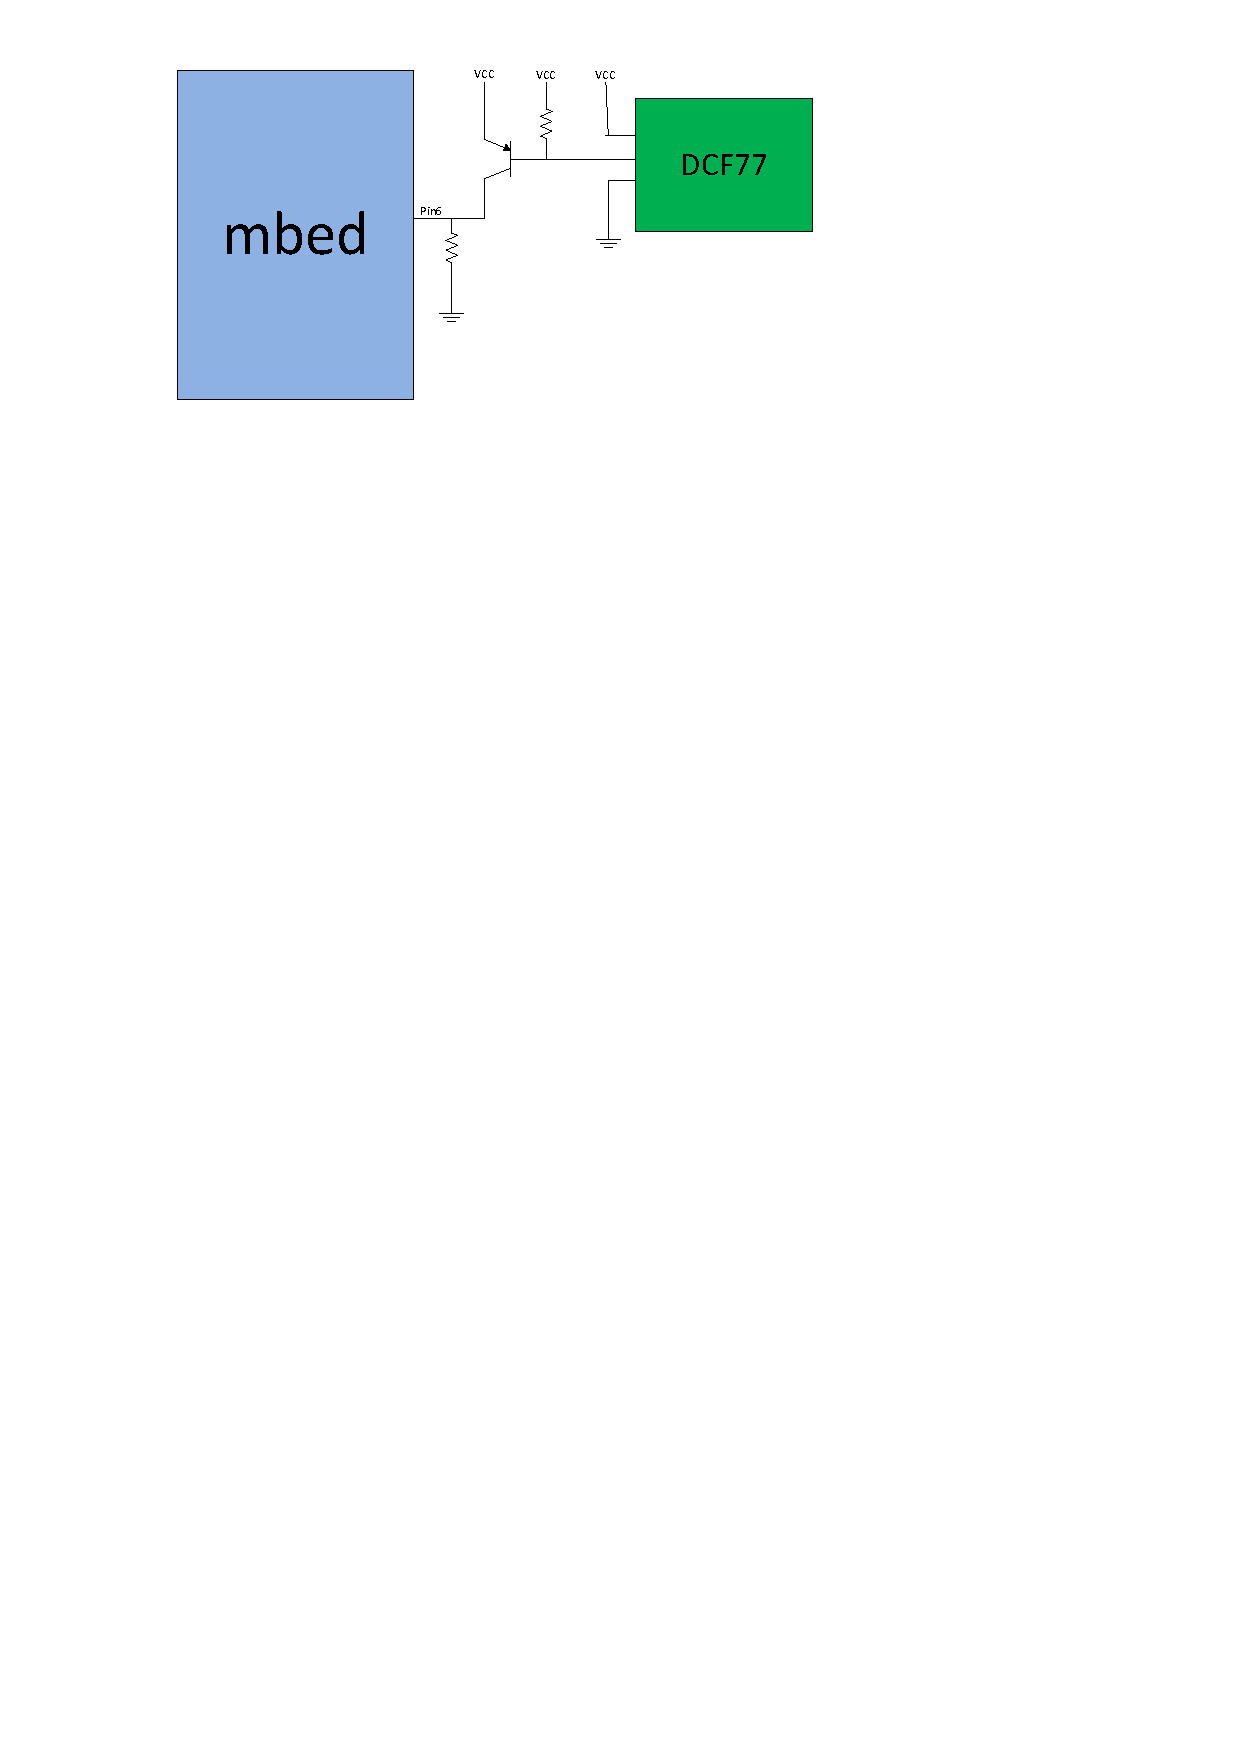
\includegraphics[width=\textwidth]{Schaltplaene/DCF77_Schaltung}
				\caption{Schaltplan DCF77}
				\label{fig:DCF77-Plan}
			\end{figure}

%			\begin{figure}[H]
%				\centering
%				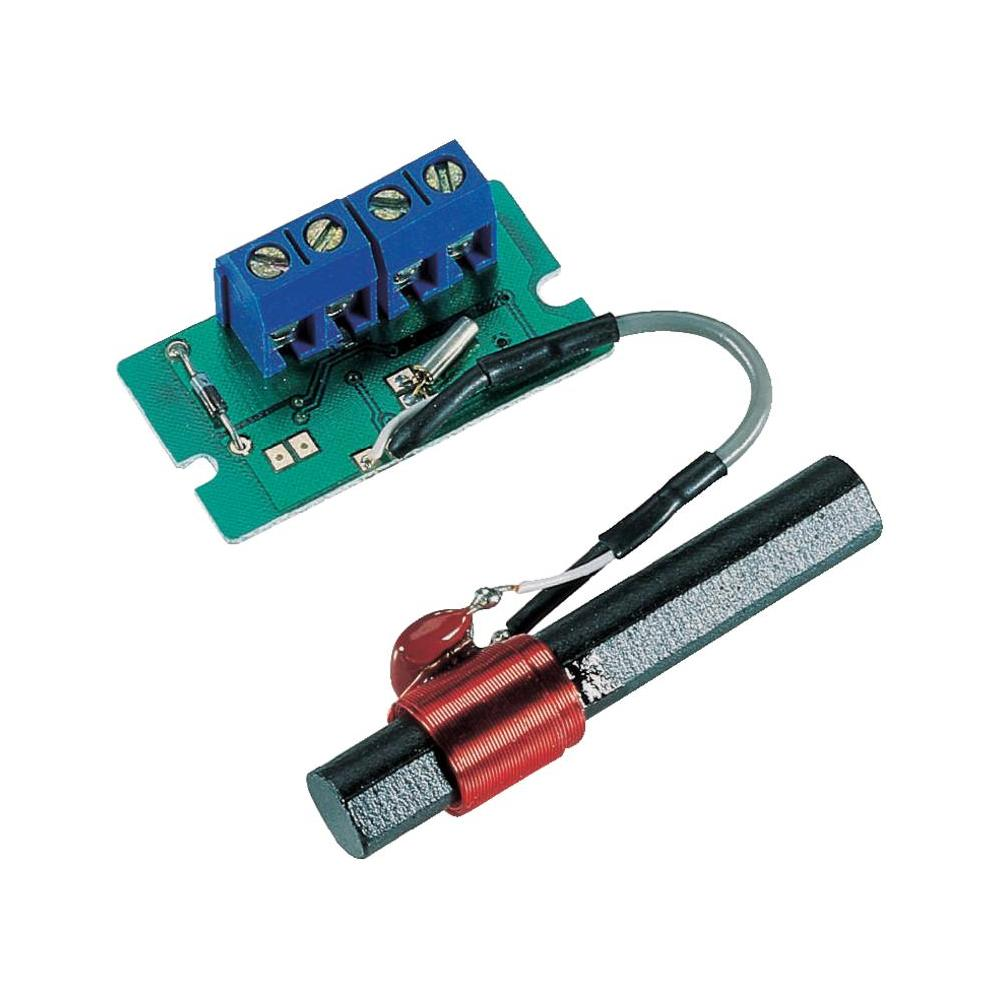
\includegraphics[width=0.7\linewidth]{Schaltplaene/DCF77}
%				\caption{Schaltplan DCF77}
%				\label{fig:DCF77-Plan}
%			\end{figure}
			
			\newpage
			Zum Ende jeder Minute fehlt eine dieser logischen Nullen. Diese lange logische eins (2 s) markiert den Beginn einer neuen Übertragung. Folgend wird zum Beginn jeder Sekunde ein Informationsbit übertragen. Eine Entscheidung, ob das Bit einer eins oder einer null entspricht, geschieht über die Länge der anliegenden logischen null. Liegt diese bei 100 ms, so ist dies als 0 zu interpretieren. Liegt diese bei 200 ms, so ist dies als 1 zu interpretieren. Damit ist das Protokoll ähnlich zum 1-Wire Protokoll, jedoch deutlich einfacher.
			
			Ein entsprechender Verlauf des Signals ist in Abbildung \ref{fig:DCF77_Impulse} zu sehen.
			
			\begin{figure}[H]
				\centering
				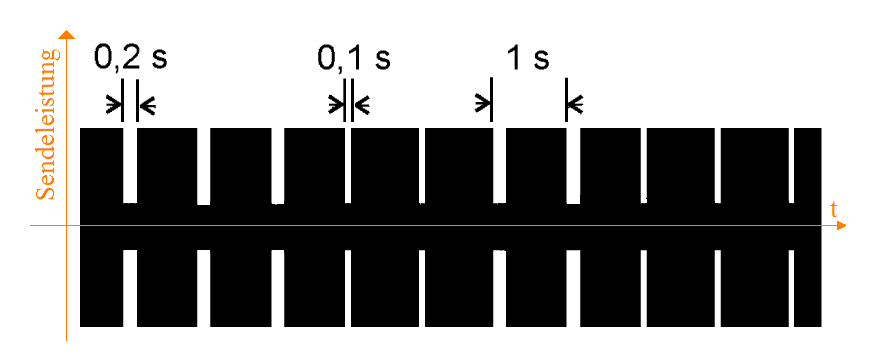
\includegraphics[width=12cm]{Grafiken/DCF77_Impulse}
				\caption[Amplitudenmodulierte Sendeleistung als Funktion der Zeit]{Amplitudenmodulierte Sendeleistung als Funktion der Zeit\protect\footnotemark}
				\label{fig:DCF77_Impulse}
			\end{figure}
			\footnotetext{Quelle: \cite{DCF77Wiki}}
			
			Letztlich können so über eine Minute 59 Bits an Informationen empfangen werden, ehe mit der langen logischen 1 ein erneuter Übertragungszyklus beginnt.
			
			\cite{DCF77Wiki}
		\subsection{Übertragene Informationen}
			In denen vom Sender ausgestrahlten 59 Bits sind kodiert verschiedene Informationen enthalten:
			
			\newpage
			\begin{itemize}
				\item Wetterinformationen der Firma MeteoTime
				\item Informationen zum Katastrophenschutz
				\item MEZ oder MESZ
				\item Uhrzeit
				\item Datum
				\item Am Ende der Stunde wird MEZ/MESZ umgestellt
				\item Am Ende der Stunde wird eine Schaltsekunde eingefügt
			\end{itemize}
			
			Die Wetterinformationen sowie die Informationen zum Katastrophenschutz sind dabei verschlüsselt und müssen über einen erwerbbaren Schlüssel dekodiert werden. Die restlichen Informationen (Uhrzeit, Datum) sind als BCD-Zahlen kodiert.
			
			Bezüglich der Uhrzeit werden die Minuten und Stunden des aktuellen Tages übertragen. Die aktuellen Sekunden können über den Beginn der Übertragung herausgefunden werden, da diese immer zur Sekunde null beginnt.
			
			Bezüglich des Datums werden der Kalendertag, der Wochentag, die Monatsnummer und das Jahr übertragen.
			
			\cite{DCF77Wiki}
		\subsection{Auswertung der Informationen}
			Die Bits samt ihren Bedeutungen sind der im Anhang dargestellten Tabelle \ref{table:DCF77Frame} zu entnehmen.
			
			Bits 0 bis 15 können dabei ignoriert werden, sofern man den für diese Informationen benötigten Schlüssel nicht besitzt.
			Die Bits 16 bis 19 können direkt ausgewertet werden, ohne eine Dekodierung vornehmen zu müssen.
			
			Letztlich muss noch das Datum und die Uhrzeit ausgewertet werden. Diese Informationen sind BCD kodiert. Am Beispiel der Minute wird gezeigt, wie diese zu dekodieren sind.
			
			Wird die Bitreihenfolge \enquote{1100101} als Bits 21 bis 27 empfangen so können hieraus die in der aktuellen Stunde verstrichenen Minuten dekodiert werden. Entsprechend der Kodierung wird jedem Bit eine spezielle Dezimalzahl zugeordnet. Die Bits müssen nun nur entsprechend der Zuordnung multipliziert werden, um die Uhrzeit herauszufinden. Am Beispiel der obigen Reihenfolge:
			
			\[ 1*1+1*2+0*4+0*8+1*10+0*20*1*40 = 53 \]
			
			Somit steht die Reihenfolge \enquote{1100101} der Bits 21 bis 27 für die Minute 53.
			
			Für die Minuten, Stunden sowie das gesamte Datum existieren jeweils Prüfbits. Diese stellen Paritätsbits einer positive Paritätsprüfung dar. Zusätzlich zu dieser schwachen Überprüfung auf Übertragungsfehler kann nach dem Dekodieren der einzelnen Datenfelder noch geprüft werden, ob diese im richtigen Wertebereich vorliegen. Am Beispiel der Minuten muss überprüft werden, ob diese im Bereich 0 bis 59 liegen.
			
			Hat die Prüfung alle Instanzen erfolgreich durchlaufen kann man relativ sicher sein, die richtigen Informationen erhalten zu haben. Sollte man den Fehler weiter minimieren wollen, so muss man mehrere Minuten das Signal empfangen und dann entsprechend vergleichen, ob jeder empfange Bitstrom gleiche Datenstempel (mit entsprechend veränderter Minute) liefert.
			
			\cite{DCF77Wiki}
		\subsection{Besonderheiten der Implementierung}
			Dadurch, dass das Signal wenigstens 38 Sekunden empfangen werden muss um eine gültige Uhrzeit zu bestimmen, wurde das gesamte Programm auf eine minimale Systemlast optimiert. Dies umfasst den besonders kritischen Empfang des Bitstrom, aber auch die Minimierung der Speicherlast.
			
			Der Empfang des Bitstroms erfolgt über Interrupts an einem Eingangspin. Diese sind so arrangiert, dass bei fallender Flanke ein Timer gestartet wird, der bei steigender Flanke angehalten und ausgewertet wird. Hat dieser Timer eine Zeit zwischen 50 und 250 ms aufgenommen, so wird das Bit entsprechend der Vorschrift geschaltet. Lief der Timer kürzer oder länger, so wird ein Fehlerfall geschaltet. Dieser kann beispielsweise auftreten, wenn schlechter Empfang vorherrscht.
			
			Diese Implementierungsart ist grundsätzlich einer Benutzung von \enquote{wait()} vorzuziehen, da mit der wait-Funktion der komplette Prozessor blockiert wird. Die Funktion \enquote{Thread::wait()} bzw. die Benutzung von Semaphoren ist hier eindeutig vorzuziehen, da diese nur den aktuellen Thread blockieren.
			
			Solange der Bitstrom (59 Bits) empfangen wird, wird die Ausführung des eigentlich aufrufenden Programms über einen Semaphor blockiert. Es sollte also darauf geachtet werden diesen Sensor in einem extra Thread laufen zu lassen, welcher blockieren kann ohne die restliche Programmausführung zu behindern.
			
			Entsprechend der Dokumentation wird am Bitstrom eine Paritätsprüfung vorgenommen. Ist diese erfolgreich, werden die Daten dekodiert und nochmals bezüglich des Wertebereichs geprüft. Lief auch hier alles erfolgreich durch, kehrt der Funktionsaufruf mit einem \enquote{true} zurück. Trat wider erwarten ein Fehler auf, wird der Empfang maximal drei mal wiederholt, ehe der Funktionsaufruf mit einem \enquote{false} zurückkehrt.
			
			Die erfolgreich gewandelte Uhrzeit kann nun über eine Funktion abgerufen werden. Mit dieser erhaltenen Information kann über eine weitere Funktion die interne \enquote{Real-Time-Clock} gesetzt werden.
	\section{Regensensor CON-REGME-24V}
		\subsection{Auswertung der Informationen}
			Der Sensor liefert nur eine sehr einfache Information. Es wird lediglich über das potentialfreie Relais bereitgestellt, ob Niederschlag vorherrscht oder nicht.
		\subsection{Besonderheiten der Implementierung}
			Der Sensor wird, sobald initialisiert, genau wie der DCF77 Schaltkreis über einen Interrupt-Pin abgefragt. Bei einer steigenden Flanke setzt das Programm intern den Wert dafür, das es Regnet auf \enquote{true}, bei einer fallenden Flanke auf \enquote{false}.
			
			Diese Vorgehensweise verringert genau wie beim Programm für den DCF77 Schaltkreis die Systemlast zu einer aktiven Abfrage enorm und der interne Zustand ist unabhängig von den Aufrufbedingungen immer aktuell.
			
			Über eine entsprechend bereitgestellte Funktion kann der aktuelle Zustand abgefragt werden.
	\section{Logging}
		\subsection{Die Logging Klasse}
		Um die empfangenen Sensordaten zu speichern und später auszuwerten wurde eine Logging-Funktion implementiert. Hierzu wurde keine neue Hardware verbaut, es handelt sich um eine reine Softwarelösung. Auf dem mbed-Entwicklungsboard befindet sich ein 2 MByte großer Flash-Speicher, der zum Protokollieren der Messwerte ausreicht.
		
		Um auch die Logging-Funktion zu kapseln wurde eine Logging-Klasse erstellt. Nach dem Erstellen eines Logging-Objektes muss nur die log() Methode aufgerufen werden um etwas zu speichern. Mit dem Erstellen eines Log-Objektes wird automatisch ein Filepointer auf die Datei \enquote{LOG.txt} geöffnet. Beim Zerstören des Objektes wird dieser wieder geschlossen.
		\subsection{Puffer Funktion}
		Ein Flash-Speicher hat nur eine begrenzte Anzahl an Schreibvorgängen pro Speicherzelle. Um diese Schreibzyklen optimal auszunutzen, wurde darauf geachtet die Schreibzugriffe gering zu halten und zugleich möglichst viel auf einmal zu schreiben.
		
		Der Flash-Speicher wurde auf 512 Byte-Blöcke formatiert. Diese werden, wenn möglich, mit einem mal voll beschrieben. Die zu schreibenden Daten werden im RAM des mbed Entwicklungsboards zwischengespeichert. Wenn über 450 Byte Gesamtgröße des Pufferarrays erreicht sind wird der gesamte Pufferspeicher auf den Flash-Speicher geschrieben.